\documentclass[border=0.8ex,svgnames,tikz]{standalone}
\usepackage{amsmath,mathtools}
\usepackage{fontspec}
\setmainfont{Source Serif 4}
\setsansfont{Source Sans 3}
\setmonofont{Source Code Pro}

\usetikzlibrary{decorations.markings}

\begin{document}
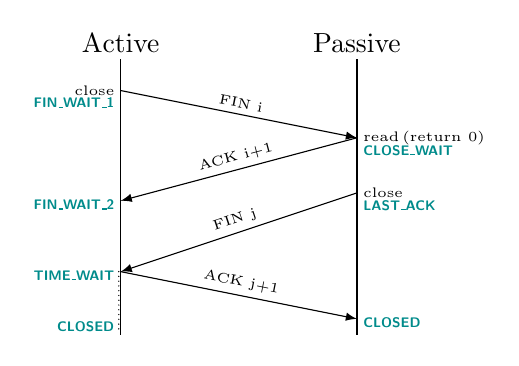
\begin{tikzpicture}[
  every label/.style={font=\tiny},
  every node/.style={inner sep=0.5ex,above,sloped,font=\tiny},
  dotted pattern/.style={
    postaction=decorate,
    decoration={
      markings,
      mark=
      between positions 0 and 1 step 0.4ex
      with
      {
        \fill[radius=0.06ex,black] (0,0) circle;
      }
    }
  },
  status node/.append style={text=DarkCyan,font=\tiny\sf\bfseries},
  ]
  \path[draw] (0,0) coordinate(active-begin)
    node[above,font=\normalsize]{Active} -- (0,-3.5);
  \path[draw] (active-begin)
    ++(0,-0.40) coordinate[label=left:{close}](active-close)
    ++(0,-1.40) coordinate(active-finwait2)
    ++(0,-0.90) coordinate(active-timewait)
    ++(0,-0.65) coordinate(active-closed);
  \path (active-close)    ++(0,-0.16) node[left,status node]{FIN\_WAIT\_1}
        (active-finwait2) ++(0,-0.05) node[left,status node]{FIN\_WAIT\_2}
        (active-timewait) ++(0,-0.05) node[left,status node]{TIME\_WAIT}
        (active-closed)   ++(0,-0.05) node[left,status node]{CLOSED};

  \path[draw] (3,0) coordinate(passive-begin)
    node[above,font=\normalsize]{Passive} -- (3,-3.5);
  \path[draw] (passive-begin)
    ++(0,-1.0) coordinate[label=right:{read\,(return 0)}](passive-read)
    ++(0,-0.7) coordinate[label=right:{close}](passive-close)
    ++(0,-1.6) coordinate(passive-closed);
  \path (passive-read)     ++(0,-0.16) node[right,status node]{CLOSE\_WAIT}
        (passive-close)    ++(0,-0.16) node[right,status node]{LAST\_ACK}
        (passive-closed)   ++(0,-0.05) node[right,status node]{CLOSED};

  \path[draw] (active-close)    edge[-latex] node{FIN i}   (passive-read)
              (passive-read)    edge[-latex] node{ACK i+1} (active-finwait2)
              (passive-close)   edge[-latex] node{FIN j}   (active-timewait)
              (active-timewait) edge[-latex] node{ACK j+1} (passive-closed);

  \path[dotted pattern] ([xshift=-0.7]active-timewait) --
  ([xshift=-0.7,yshift=-3]active-closed);
\end{tikzpicture}
\end{document}
